%!TEX program = xelatex
% 完整编译方法 1 pdflatex -> bibtex -> pdflatex -> pdflatex
% 完整编译方法 2: xelatex -> bibtex -> xelatex -> xelatex
\documentclass[lang=cn,11pt,numbers]{elegantpaper}
\usepackage{float}
%% 去掉图标的冒号
\usepackage{caption}
\DeclareCaptionLabelSeparator{twospace}{\ ~}   %%这三条语句即可
\captionsetup{labelsep=twospace}
%%使用\upcite{}上标参考文献 
\newcommand{\upcite}[1]{\textsuperscript{\textsuperscript{\cite{#1}}}}

\title{商业信息系统(BIS)分析}
\author{0121710880223 - 软件工程1702 - 刘佳迎}

%\institute{\href{https://elegantlatex.org/}{Elegant\LaTeX{} 项目组}}

% 不需要版本信息,直接注释即可
%\version{0.07}
% 不需要时间信息的话,需要把 \today 删除。
\date{\today}
\geometry{a4paper,scale=0.8}
\usepackage{indentfirst}\setlength{\parindent}{2em}

\begin{document}

\maketitle

\begin {abstract} 

随着互联网与云计算技术的发展,电子商务已经达到商务智能(BI)新高度。 在云计算环
境下,商务智能系统能够突出面向用户、易于访问、可自助编程的特点,本文针对以上特点分析了商务智能系统的内涵,
并针对现有技术,罗列分析了商务信息系统的知名产品的特点。
\keywords 
{ 数据库技术 \quad}
\end{abstract}


\section{什么是商业信息系统(BIS)}

BIS全称为Business Information System, 商业信息系统,它是商业需求和计算机编程的桥梁。
商务智能系统雏形是基于事务的管理信息系统,后来
出现了高级管理信息系统,在分析和处理综合性与复杂性
问题的能力上有了进一步的提高。 在管理信息系统(MIS)
的基础上,又出现了决策支持系统,最终演变成商务智能
系统。因此,商务智能系统是依赖于原始海量业务数据的,
并对这些数据进行存储及加工处理的,可以为决策者提供
智能服务的管理信息系统。 它的核心仍然是数据仓库系
统,需要先收集大量的数据并对其整理形成可供使用的数
据, 然后把这些经过预处理的数据进行加工转化成信息,
形成的最终智慧产品用于指导商务实践\upcite{one}。 

IBM 公司曾经提出过 一 个 体 系 结 构\upcite{two},主要有下面的几个 组成部分:外
部数据源 、数据仓 库 建 模 和 构 造工具 、数据管 理、访 问 工
具 、决 策 支 持 工 具 、商 务 智 能 应 用 、元 数 据 管 理 ,相 互 间
通过体系内的协作可以提供数据分析与管理、知识发现等功能。
众所周知,全球经济一体化格局下,商务智能系统越来越需要面向全球范围和全域视野的用户经营管理与辅
助决策需求,随之而来,系统建设的硬件、网络资源耗费急剧增长,软件架构日益庞大,以知识与方法为核心的智库
趋于复杂。 因此,云计算技术将系统的软硬件资源全部构建于云端,使客户端实现“瘦身”,是新一代商务智能发展
的重要出路。





我们再举一个实例,就是目前即将在中国流行,在西方已经很流行的CRM管理系统。

客户关系管理(Customer Relationship Management,CRM),是现代管理科学与先进信息技术结合的产物,是企业树立“以客户为中心”的发展战略,并在此基础上开展的包括判断、选择、争取、发展和保持客户所实施的全部商业过程;是企业以客户关系为重点,通过再造企业组织体系和优化业务流程,展开系统的客户研究,提高客户满意度和忠诚度,提高运营效率和利润收益的工作实践;也是企业为最终实现电子化、运营目标所创造和使用的软硬件系统及集成的管理方法、解决方案的总和。

一套CRM系统大都具备市场管理、销售管理、销售支持与服务和竞争对象记录与分析的功能。


\begin{figure}[H]
	\centering
	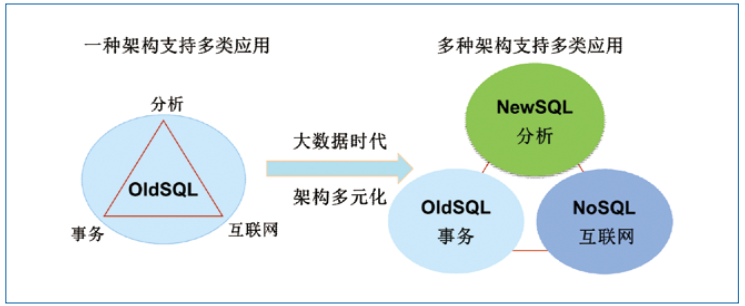
\includegraphics{Snipaste_2019-09-04_22-27-14.png}
	\caption{ 大数据引发的数据库架构变革 \label{fig:2}}
\end{figure}

\begin{table}[H]
  
  \centering
  \caption{大数据带来的数据库产品创新示例 \label{tab:reg}}
  \setlength{\tabcolsep}{7mm}{  %%调整表格宽度
    \begin{tabular}{cccccc}
    \toprule
    NewSQL      &       NoSQL        &       OldSQL     \\
    \midrule
    GBase 8a & Hadoop & TimesTen \\
    Greenplum & HBase & Altibase\\
    Vertica & Bigtable  & SolidDB\\
    AsterData & Cassandra & Exadata\\
    Sybase IQ & Dynamo & Netezza\\
    F1/Spanner & Dremel & Teradata\\
    \bottomrule
    
    \end{tabular} }
\end{table}%

\nocite{*}
\bibliography{wpref}

\end{document}
